\documentclass[tikz]{standalone}
\usepackage{pgfplots}
\pgfplotsset{compat=newest}
\pgfplotsset{every axis legend/.append style={%
cells={anchor=west}}
}
\usepgfplotslibrary{polar}
\usetikzlibrary{arrows}
\tikzset{>=stealth'}

\begin{document}
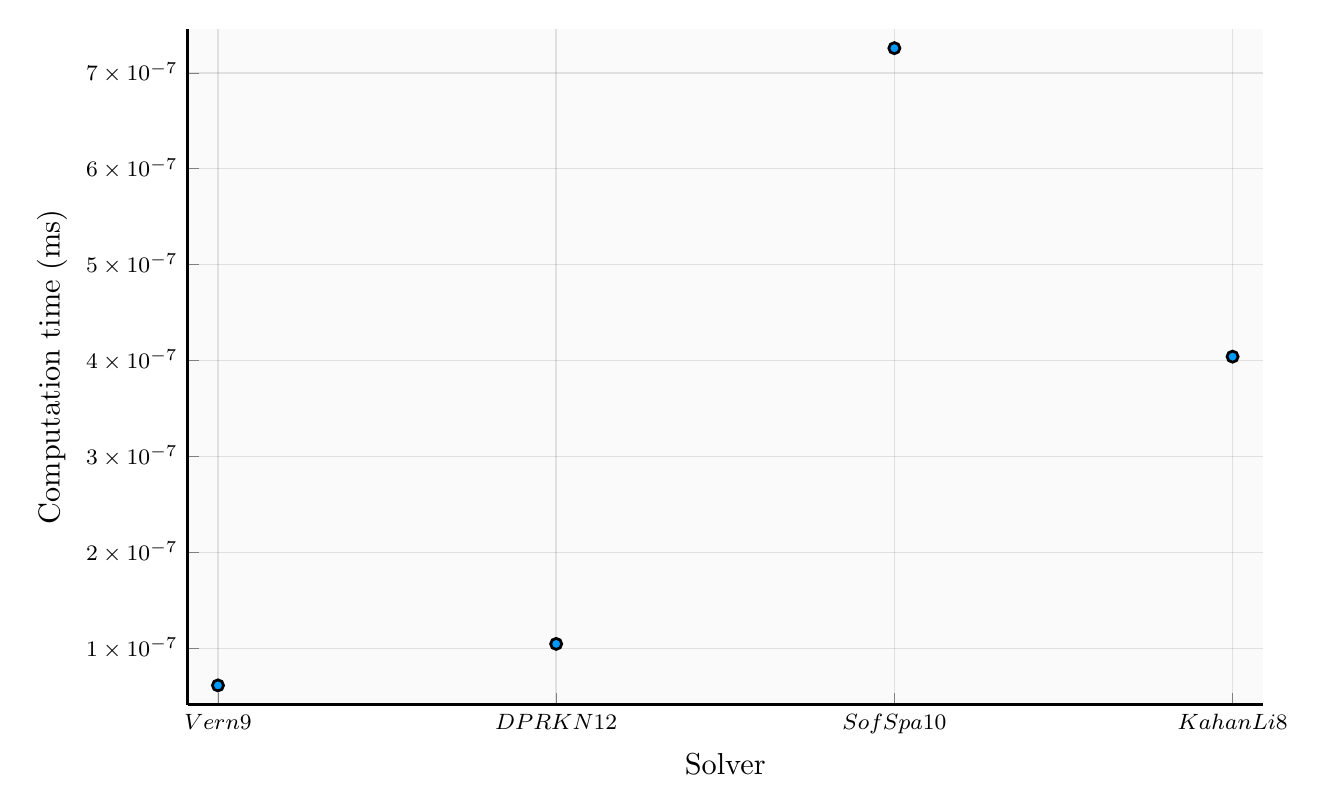
\begin{tikzpicture}[]
\begin{axis}[height = {101.6mm}, ylabel = {Computation time (ms)}, xmin = {0.41000000000000003}, xmax = {3.59}, ymax = {7.4572075322e-7}, xlabel = {Solver}, unbounded coords=jump,scaled x ticks = false,xlabel style = {font = {\fontsize{11 pt}{14.3 pt}\selectfont}, color = {rgb,1:red,0.00000000;green,0.00000000;blue,0.00000000}, draw opacity = 1.0, rotate = 0.0},xmajorgrids = true,xtick = {0.5,1.5,2.5,3.5},xticklabels = {$Vern9$,$DPRKN12$,$SofSpa10$,$KahanLi8$},xtick align = inside,xticklabel style = {font = {\fontsize{8 pt}{10.4 pt}\selectfont}, color = {rgb,1:red,0.00000000;green,0.00000000;blue,0.00000000}, draw opacity = 1.0, rotate = 0.0},x grid style = {color = {rgb,1:red,0.00000000;green,0.00000000;blue,0.00000000},
draw opacity = 0.1,
line width = 0.5,
solid},axis x line* = left,x axis line style = {color = {rgb,1:red,0.00000000;green,0.00000000;blue,0.00000000},
draw opacity = 1.0,
line width = 1,
solid},scaled y ticks = false,ylabel style = {font = {\fontsize{11 pt}{14.3 pt}\selectfont}, color = {rgb,1:red,0.00000000;green,0.00000000;blue,0.00000000}, draw opacity = 1.0, rotate = 0.0},ymajorgrids = true,ytick = {1.0e-7,2.0e-7,3.0e-7,4.0e-7,5.0e-7,6.0e-7,7.0e-7},yticklabels = {$1\times10^{-7}$,$2\times10^{-7}$,$3\times10^{-7}$,$4\times10^{-7}$,$5\times10^{-7}$,$6\times10^{-7}$,$7\times10^{-7}$},ytick align = inside,yticklabel style = {font = {\fontsize{8 pt}{10.4 pt}\selectfont}, color = {rgb,1:red,0.00000000;green,0.00000000;blue,0.00000000}, draw opacity = 1.0, rotate = 0.0},y grid style = {color = {rgb,1:red,0.00000000;green,0.00000000;blue,0.00000000},
draw opacity = 0.1,
line width = 0.5,
solid},axis y line* = left,y axis line style = {color = {rgb,1:red,0.00000000;green,0.00000000;blue,0.00000000},
draw opacity = 1.0,
line width = 1,
solid},    xshift = 0.0mm,
    yshift = 0.0mm,
    axis background/.style={fill={rgb,1:red,0.98039216;green,0.98039216;blue,0.98039216}}
,legend style = {color = {rgb,1:red,0.00000000;green,0.00000000;blue,0.00000000},
draw opacity = 1.0,
line width = 1,
solid,fill = {rgb,1:red,0.98039216;green,0.98039216;blue,0.98039216},font = {\fontsize{8 pt}{10.4 pt}\selectfont}},colorbar style={title=}, ymin = {4.1285060780000005e-8}, width = {152.4mm}]\addplot+[draw=none, color = {rgb,1:red,0.00000000;green,0.60560316;blue,0.97868012},
draw opacity = 1.0,
line width = 0,
solid,mark = *,
mark size = 2.0,
mark options = {
    color = {rgb,1:red,0.00000000;green,0.00000000;blue,0.00000000}, draw opacity = 1.0,
    fill = {rgb,1:red,0.00000000;green,0.60560316;blue,0.97868012}, fill opacity = 1.0,
    line width = 1,
    rotate = 0,
    solid
},forget plot] coordinates {
(0.5, 6.122192e-8)
(1.5, 1.0450410899999999e-7)
(2.5, 7.25783894e-7)
(3.5, 4.0406350400000004e-7)
};
\end{axis}

\end{tikzpicture}
\end{document}
